% Pontos A(0,0), B(2,0), C(3,0)
% 4kN/m aplicada para baixo entre B e C
% Engastado em A

\documentclass[tikz]{standalone}
\usepackage{stanli}
\usetikzlibrary{calc}

\begin{document}
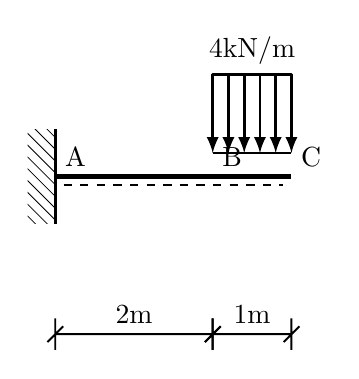
\begin{tikzpicture}
    % Definição dos pontos
    \point{A}{0}{0}
    \point{B}{2}{0}
    \point{C}{3}{0}

    % Definição dos apoios
    % Engastado em A (parede à esquerda: rotação = -90)
    \support{3}{A}[-90]

    % Definição da viga
    \beam{1}{A}{C}

    % Carga distribuída
    % 4kN/m para baixo entre B e C
    \lineload{1}{B}{C}

    % Notações e Etiquetas
    \notation{1}{A}{A}[above right]
    \notation{1}{B}{B}[above right]
    \notation{1}{C}{C}[above right]
    
    % Regra: carga distribuída utiliza [above=13mm]
    \notation{5}{B}{C}[4kN/m][.5][above=13mm]

    % Dimensionamento
    % Offset negativo para ficar abaixo da viga
    \dimensioning{1}{A}{B}{-20mm}[2m]
    \dimensioning{1}{B}{C}{-20mm}[1m]
\end{tikzpicture}
\end{document}